\let\negmedspace\undefined
\let\negthickspace\undefined
\documentclass[journal]{IEEEtran}
\usepackage[a5paper, margin=10mm, onecolumn]{geometry}
%\usepackage{lmodern} % Ensure lmodern is loaded for pdflatex
\usepackage{tfrupee} % Include tfrupee package

\setlength{\headheight}{1cm} % Set the height of the header box
\setlength{\headsep}{0mm}     % Set the distance between the header box and the top of the text

\usepackage{gvv-book}
\usepackage{gvv}
\usepackage{cite}
\usepackage{amsmath,amssymb,amsfonts,amsthm}
\usepackage{algorithmic}
\usepackage{graphicx}
\usepackage{textcomp}
\usepackage{xcolor}
\usepackage{txfonts}
\usepackage{listings}
\usepackage{enumitem}
\usepackage{mathtools}
\usepackage{gensymb}
\usepackage{comment}
\usepackage[breaklinks=true]{hyperref}
\usepackage{tkz-euclide} 
\usepackage{listings}
% \usepackage{gvv}                                        
\def\inputGnumericTable{}                                 
\usepackage[latin1]{inputenc}                                
\usepackage{color}                                            
\usepackage{array}                                            
\usepackage{longtable}                                       
\usepackage{calc}                                             
\usepackage{multirow}                                         
\usepackage{hhline}                                           
\usepackage{ifthen}                                           
\usepackage{lscape}
\begin{document}

\bibliographystyle{IEEEtran}
\vspace{3cm}

\title{4.13.33}
\author{EE25btech11028 - J.Navya sri}
% \maketitle
% \newpage
% \bigskip
{\let\newpage\relax\maketitle}


\textbf{Question:} \\
Find the locus of a variable point \(\myvec{P} = \myvec{(x, y)}\) whose distance from the point \(\myvec{A} = \myvec{(-2, 0)}\) is 
\(\dfrac{2}{3}\) times its distance from the line \(x = -\dfrac{9}{2}\).

\bigskip

\textbf{Solution:} \\
Let
\[
\myvec{x}=\myvec{x\\[4pt]y},\qquad
\myvec{a}=\myvec{-2\\[4pt]0},\qquad
\myvec{n}=\myvec{1\\[4pt]0},\qquad
c=\frac{9}{2}.
\]

Distance condition (given):
\begin{equation}
\label{eq:dist}
\left\lVert \myvec{x}-\myvec{a} \right\rVert
= \frac{2}{3}\,\big|\myvec{n}^T\myvec{x}+c\big|.
\end{equation}

Square both sides:
\begin{equation}
\label{eq:squared}
(\myvec{x}-\myvec{a})^T(\myvec{x}-\myvec{a})
= \frac{4}{9}\big(\myvec{n}^T\myvec{x}+c\big)^2.
\end{equation}

Evaluate each side in coordinates:
\begin{align}
(x+2)^2 + y^2
&= \frac{4}{9}\!\left(x+\frac{9}{2}\right)^{\!2} \\
x^2+4x+4 + y^2
&= \frac{4}{9}x^2 + 4x + 9 \\
\text{(cancel }4x\text{ on both sides)}\qquad
x^2 + 4 + y^2
&= \frac{4}{9}x^2 + 9
\end{align}

Multiply both sides by $9$:
\[
9x^2 + 36 + 9y^2 = 4x^2 + 81
\]
\[
\Rightarrow 5x^2 + 9y^2 = 45.
\]

Divide by $45$ to get standard form:
\begin{equation}
\boxed{\;\dfrac{x^2}{9} + \dfrac{y^2}{5} = 1\;}
\end{equation}

Thus the locus is an ellipse centered at the origin with semi-axes $3$ (along $x$) and $\sqrt{5}$ (along $y$).

\textbf{Graph presentation:}
\begin{figure}[H]
\begin{center}
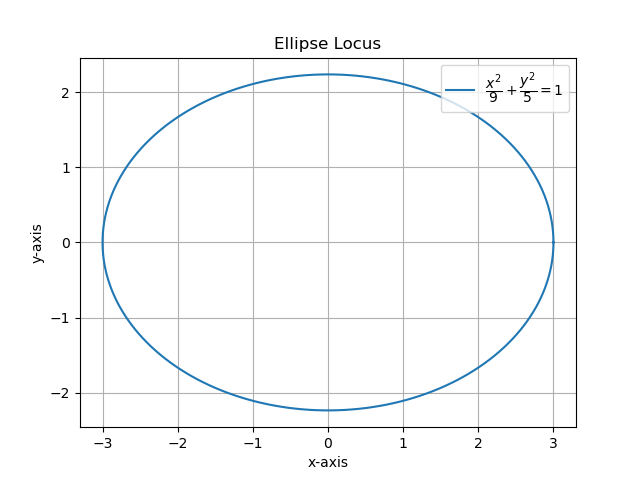
\includegraphics[width=0.6\columnwidth]{figs/fig9.png}
\end{center}
\caption{}
\label{fig:Fig}
\end{figure}
\end{document}